\subsection{Extra features}
\subsubsection{Security: reCAPTCHA}
To prevent bots abusing our service or ddos attack, we require user
to pass Google reCAPTCHA before login / sign up.
As shown in figure \ref{fig:non_user_req}, user are not able to sign in without completing the reCAPTCHA.

Note: User cannot bypass this even if they hack the frontend, as the reCAPTCHA token will be
verified in the backend.
\subsubsection{Security: password hashing}
To prevent password leak and to protect user privacy, we hash the password when
user sign up. As shown in figure \ref{fig:pw_hashing}, the password \verb|csci_2720| became a long
encrypted string, which can only be verified with our secret key.
\begin{figure}[h]
    \centering
    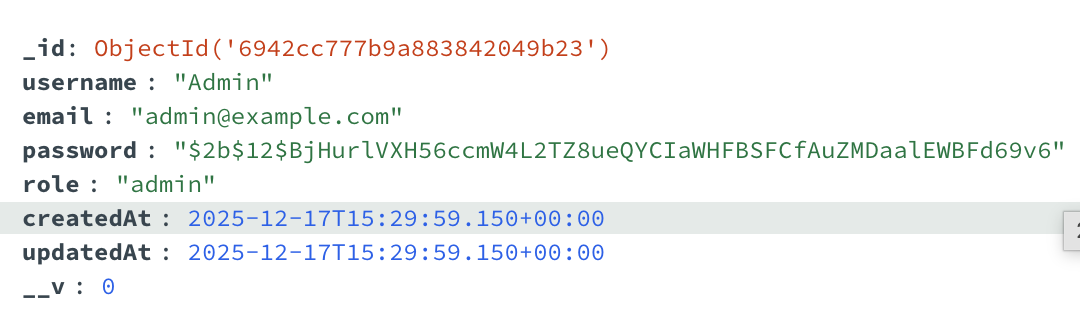
\includegraphics[width=0.8\textwidth]{figures/pw_hashing.png}
    \caption{Password hashing}
    \label{fig:pw_hashing}
\end{figure}

\subsubsection{Security: token and admin authorization}
While we use browser local storage to store user login status, we know it is not safe
as frontend data can be easily modified. To prevent malicious attempt, we store a 
token in user's local storage when they login. All attempts to assess the server must
first pass through our \verb|require-auth| middleware with the token. (See figure \ref{subfig:security_token})
You can try this by clearing browser data after login, then navigate different pages.
Don't refresh the page as that will send you to back to authentication.

On top of that, admin-only routes has to pass through an addition
\verb|require-admin| middleware with their userID. It will be compared with the database
to check if they are really admin.  (See figure \ref{subfig:security_admin})
You can try this by changing your role from "admin" to "user" on MongoDB Compass after
logging in as an admin.

\begin{figure}[h]
    \centering
    \begin{subfigure}{0.8\textwidth}
        \centering
        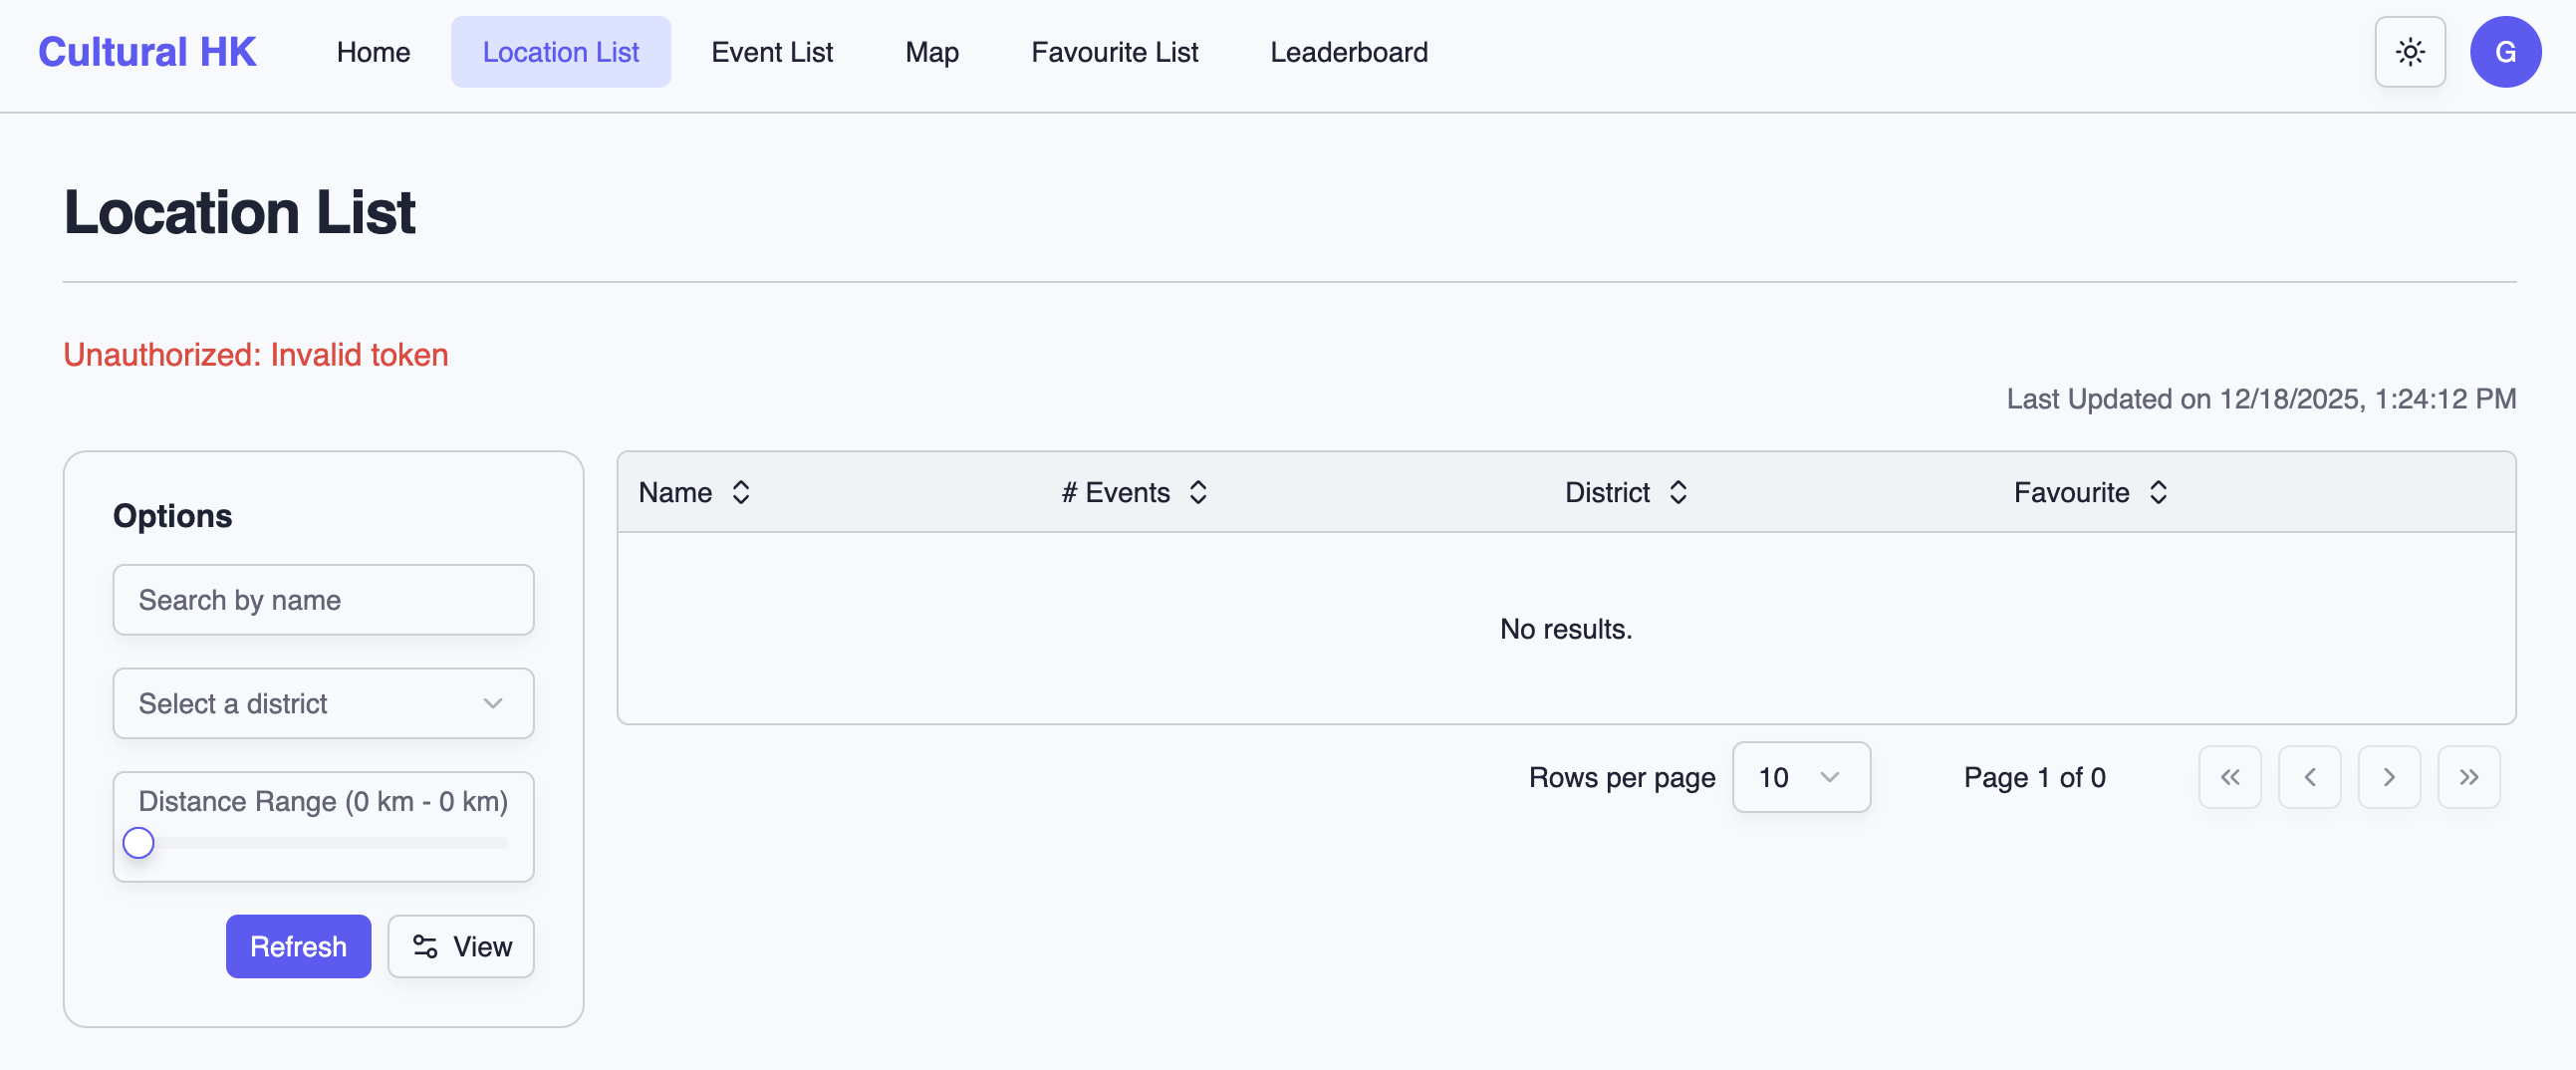
\includegraphics[width=\textwidth]{figures/security_token.png}
        \caption{User access to server rejected without valid token}
        \label{subfig:security_token}
    \end{subfigure}
    \begin{subfigure}{0.8\textwidth}
        \centering
        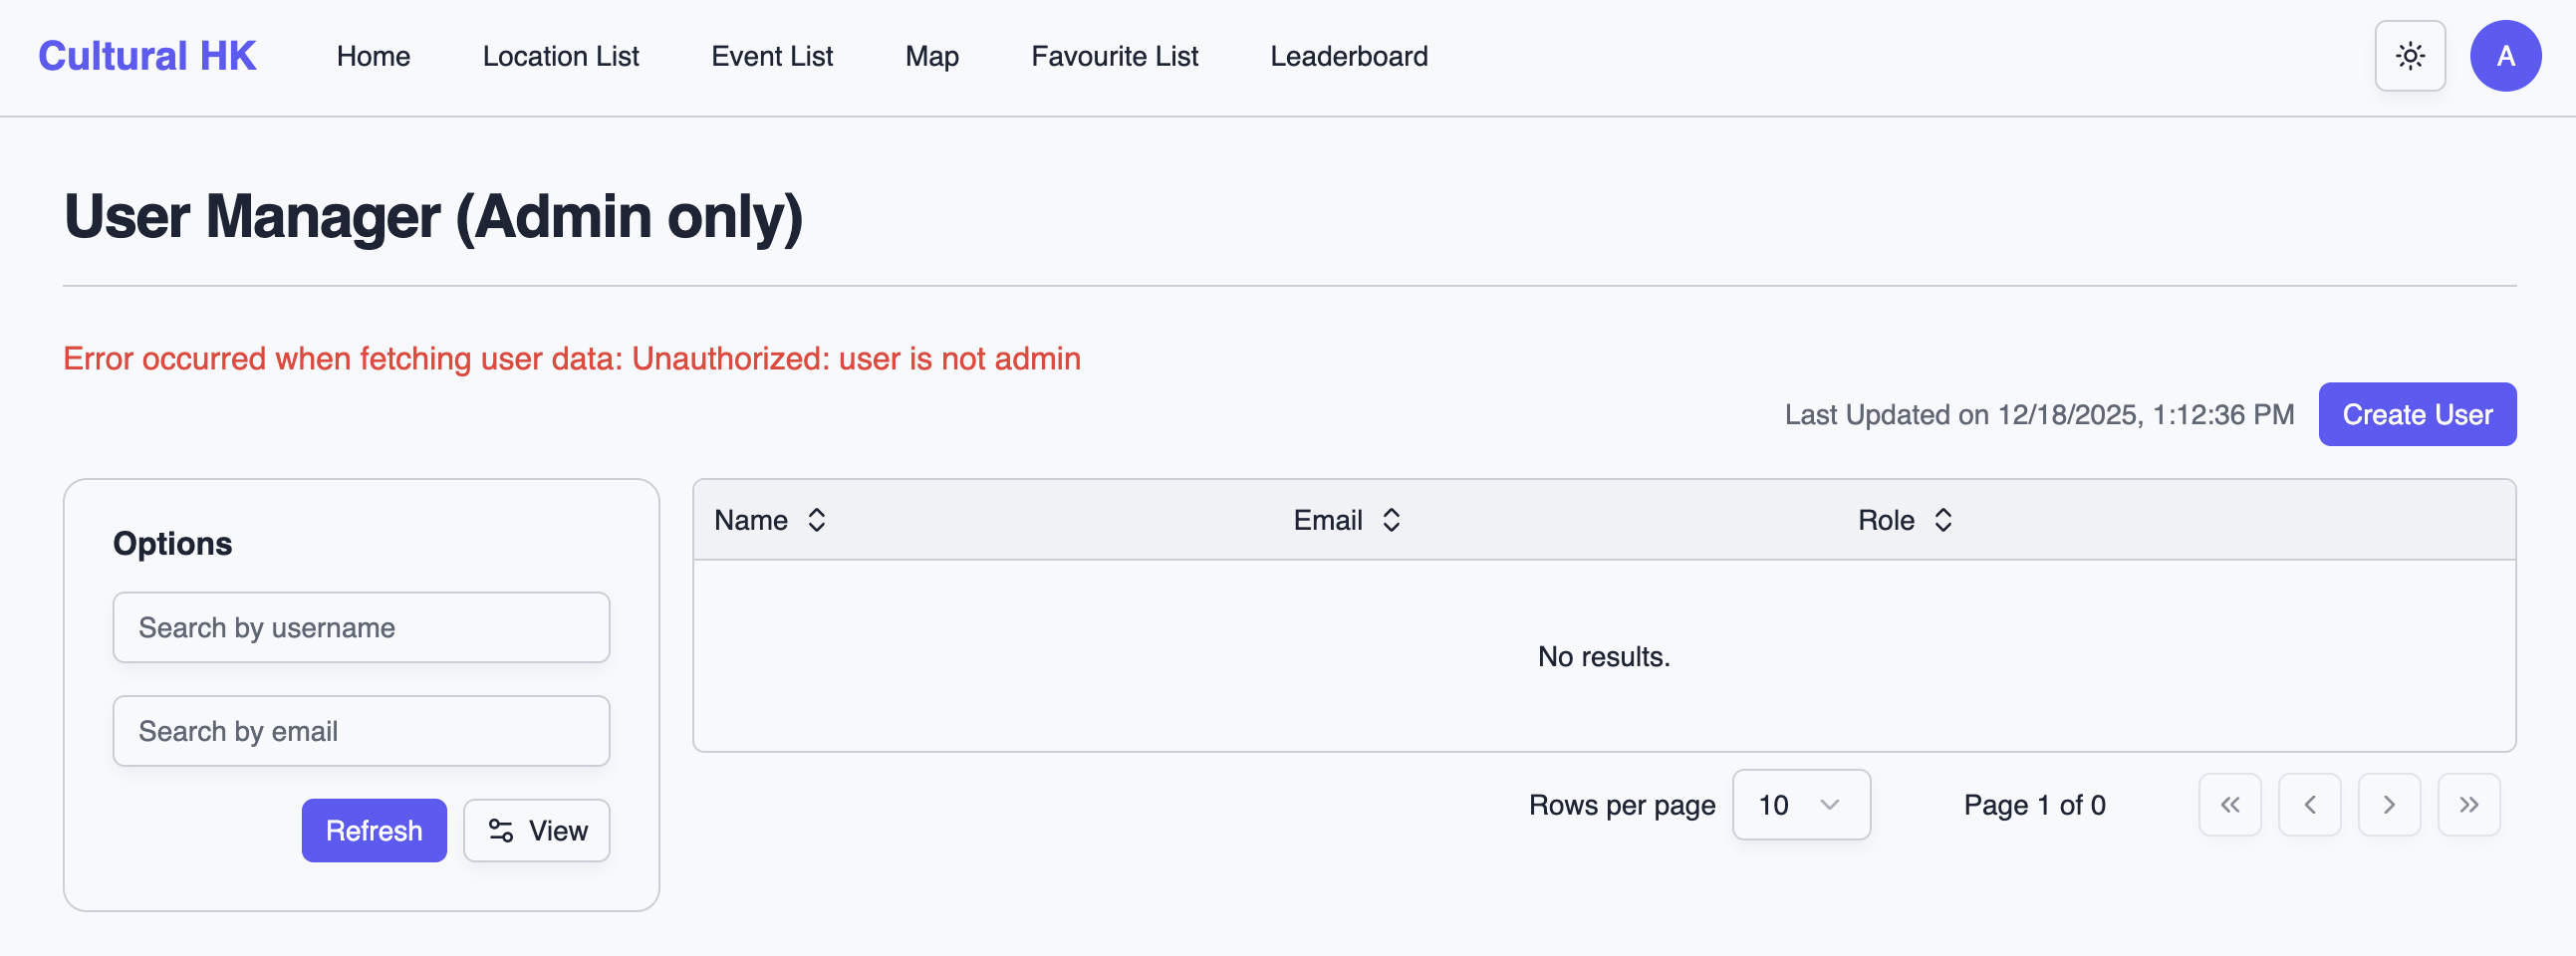
\includegraphics[width=\textwidth]{figures/security_admin.png}
        \caption{User access to admin-only page rejected due to invalid admin user ID}
        \label{subfig:security_admin}
    \end{subfigure}
    \caption{}
    \label{fig:security_token_and_admin}
\end{figure}